A software framework is a repository of reusable and adaptable software components embedded within a pre-defined architecture that is optimized for applications in a certain domain (see figure \ref{fig:SwFwConcept}).

\begin{figure}[ht]
 \centering
 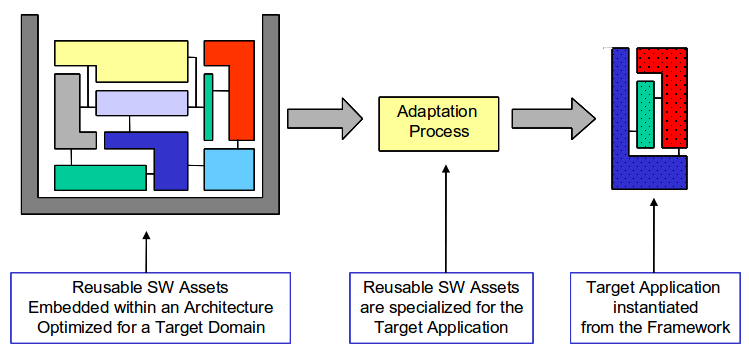
\includegraphics[scale=0.4,keepaspectratio=true]{SwFwConcept.png}
 \caption{Software Framework Concept}
 \label{fig:SwFwConcept}
\end{figure}

The framework components are reusable in the sense that they encapsulate behaviour which is common to all (or at least a large number of) applications within the framework's domain.

To reuse a software components means to use it in different operational contexts. 
In practice, varying operational contexts always impose different requirements. 
Hence, reuse requires that the reusable components be \textit{adaptable} to different requirements. 
In this sense, adaptability is the key to reusability. 
For this reason, framework components offer \textit{adaptation points} where their behaviour can be modified to match the needs of specific applications.

Framework components are embedded within a pre-defined architecture in the sense that the framework does not simply specify individual components but it also specifies their mutual relationships. 
Thus, the unit of reuse of a software framework is not a component but rather a group of cooperating components which, taken together, support the implementation of some functionality that is important within the framework domain. 

Software frameworks encourage this higher granularity of reuse by being organized as a bundle of functionalities that users can choose to include in their applications. 
Inclusion of a functionality implies that a whole set of cooperating components and interfaces is imported into the application. 

In the service-oriented concept underlying the CORDET Framework, the functionalities supported by the framework are the “services” as defined in the next section.

The \textit{domain} of a framework is the set of applications whose instantiation is supported by the framework. The domain of the CORDET Framework are the applications which comply with the CORDET service Concept introduced in section \ref{sec:ServConcept}.

